%%%%%%%%%%%%%%%%%%%%%%%%%%%%%%%%%%%%%%%%%%%%%%%%%%%%%%%%
%%%%%%%%%%%%%%%%%%%%%%%%%%%%%%%%%%%%%%%%%%%%%%%%%%%%%%%%
\section[CMS]{The CMS experiment at LHC}
\setcounter{tocdepth}{2}

\begin{frame}{}
The CMS experiment at LHC
\end{frame}

\subsection{CMS}

\begin{frame}{LHC}
\vspace{-.2cm}

\begin{columns}
\begin{column}{.50\textwidth}
\begin{figure}[!Hhtbp]
  \begin{center}
    \includegraphics[width=1.0\textwidth]{lhc_underground.jpg}
  \end{center}
\end{figure}
\vspace{-.2cm}
\begin{block}{}
\begin{itemize}\scriptsize
\item Proton and heavy ion collider
\item 27 km of circumference, 100 m underground
\item 1232 superconductor magnets at 1.9 K with a magnetic field of 8.33 T
\item Run 1: 4 TeV/proton
\item Run 2: 6.5 TeV/proton, started last June
\end{itemize}
\end{block}
\end{column}

\begin{column}{.50\textwidth}
\begin{block}{}
\begin{itemize}\scriptsize
\item In run 1: Around 1000 proton bunches, spaced 50 ns $\to$ 20 millions of collisions / s
\item Main experiments:
  \begin{itemize}\tiny
  \item Generic purpose: ATLAS and CMS
  \item Beauty physics: LHCb
  \item Quark-Gluon plasma: ALICE
  \item Forward physics: LHCf, TOTEM
  \end{itemize}
\end{itemize}
\end{block}
\vspace{-.2cm}
\begin{figure}[!Hhtbp]
  \begin{center}
    \includegraphics[width=1.0\textwidth]{lhc_hall_1.jpg}
  \end{center}
\end{figure}
\end{column}
\end{columns}

\end{frame}


\begin{frame}{}
\vspace{-.2cm}

\begin{columns}
\begin{column}{.50\textwidth}
\begin{figure}[!Hhtbp]
  \begin{center}
    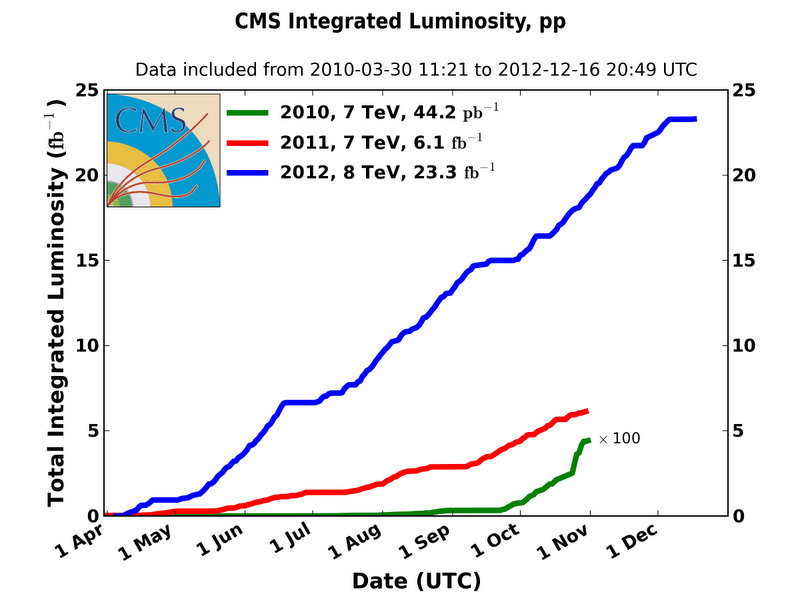
\includegraphics[width=1.0\textwidth]{../figs/cms-int-10to12.jpg}
    %\caption{CMS integrated luminosity for proton-proton collisions delivered by LHC. }
    %\label{fig:CMSlumi}
  \end{center}
\end{figure}
\vspace{-.5cm}
\begin{figure}[!Hhtbp]
  \begin{center}
    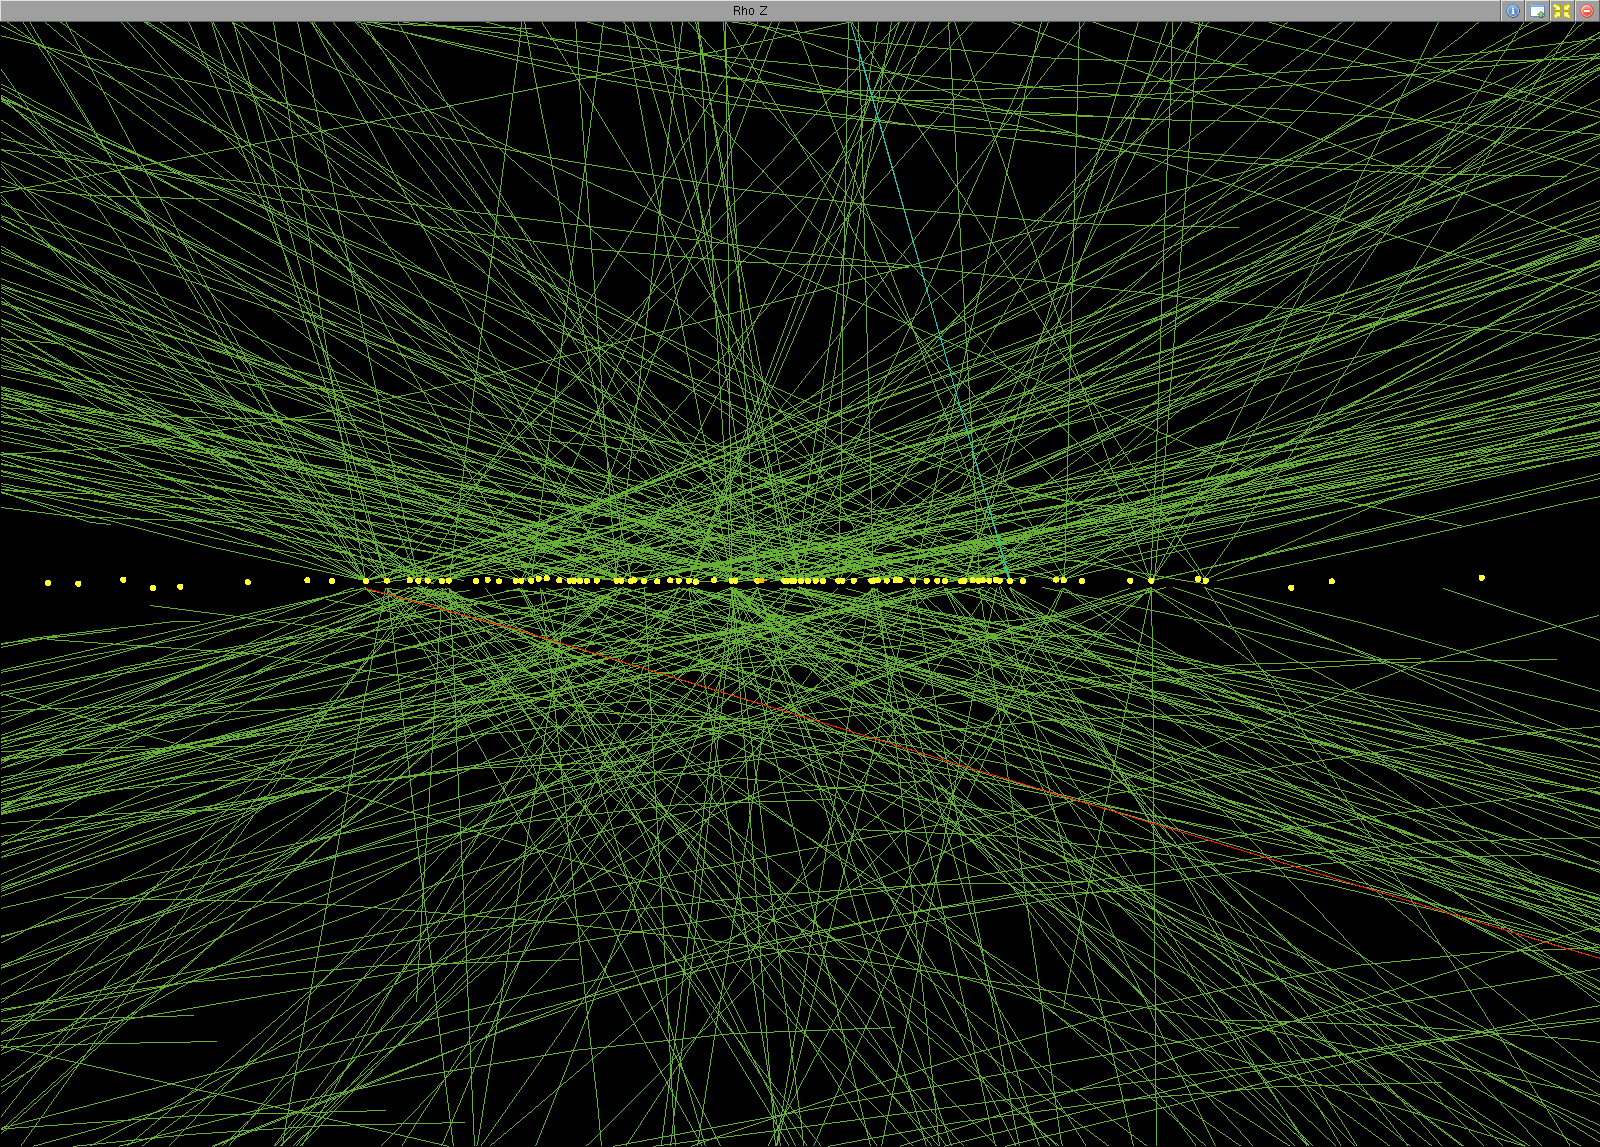
\includegraphics[width=1.0\textwidth]{../figs/pileup.png}
    %\caption{High pile-up event (78 interactions) seen by CMS detector. Event 35655522, from 198609 run, lumi 56, recorded on 2012.}% Image credit: Andre Holzner }                                        
    %\label{fig:pileup}
  \end{center}
\end{figure}
\end{column}

\begin{column}{.50\textwidth}
\begin{block}{}
\begin{equation*}
  L=\frac{k_{b}N_{b}^{2}f_{rev}}{4\pi\sigma^{*}_{x}\sigma^{*}_{y}}R                                     
\end{equation*}
\begin{equation*}
  N_{events}=L\times \sigma_{process} \times \epsilon
\end{equation*}
\end{block}

\tiny{
%\begin{table}[htbH]
\begin{center}
%\resizebox{\textwidth}{!}{
\begin{tabular}{|c|c c|}
\hline
 & 2012 & Nominal \\
\hline
Energy [GeV]& 4000 & 7000 \\
Inst. Lumi. [$\text{cm}^{-2}\text{s}^{-1}$] & 7.54$\times10^{33}$ & $10^{34}$ \\
$k_{b}$ Number of bunches & 1374 & 2808 \\
Bunch spacing [ns] & 50 & 25 \\
\hline
\end{tabular}
%}
\end{center}
%\end{table}
}%

\begin{block}{}
\begin{itemize}\scriptsize
\item Increasing the recorded luminosity $\to$ higher sensitivity to rare processes.
\item Run 1: 19.7 fb$^{-1}$ in 2012 \MVAt~8 TeV
\end{itemize}
\end{block}
\begin{block}{}
\scriptsize PileUp: 20 interactions per crossing during 2012
\end{block}
\end{column}
\end{columns}

\end{frame}

\begin{frame}{CMS: Compact Muon Solenoid}
\vspace{-.2cm}

\begin{figure}[!Hhtbp]
  \begin{center}
    \includegraphics[width=\textwidth]{cms_det.png}
  \end{center}
\end{figure}

\end{frame}


\begin{frame}{Sub-systems}
\vspace{-.2cm}
\begin{figure}[!Hhtbp]
  \begin{center}
    \includegraphics[width=0.85\textwidth]{SubDet.jpg}
    %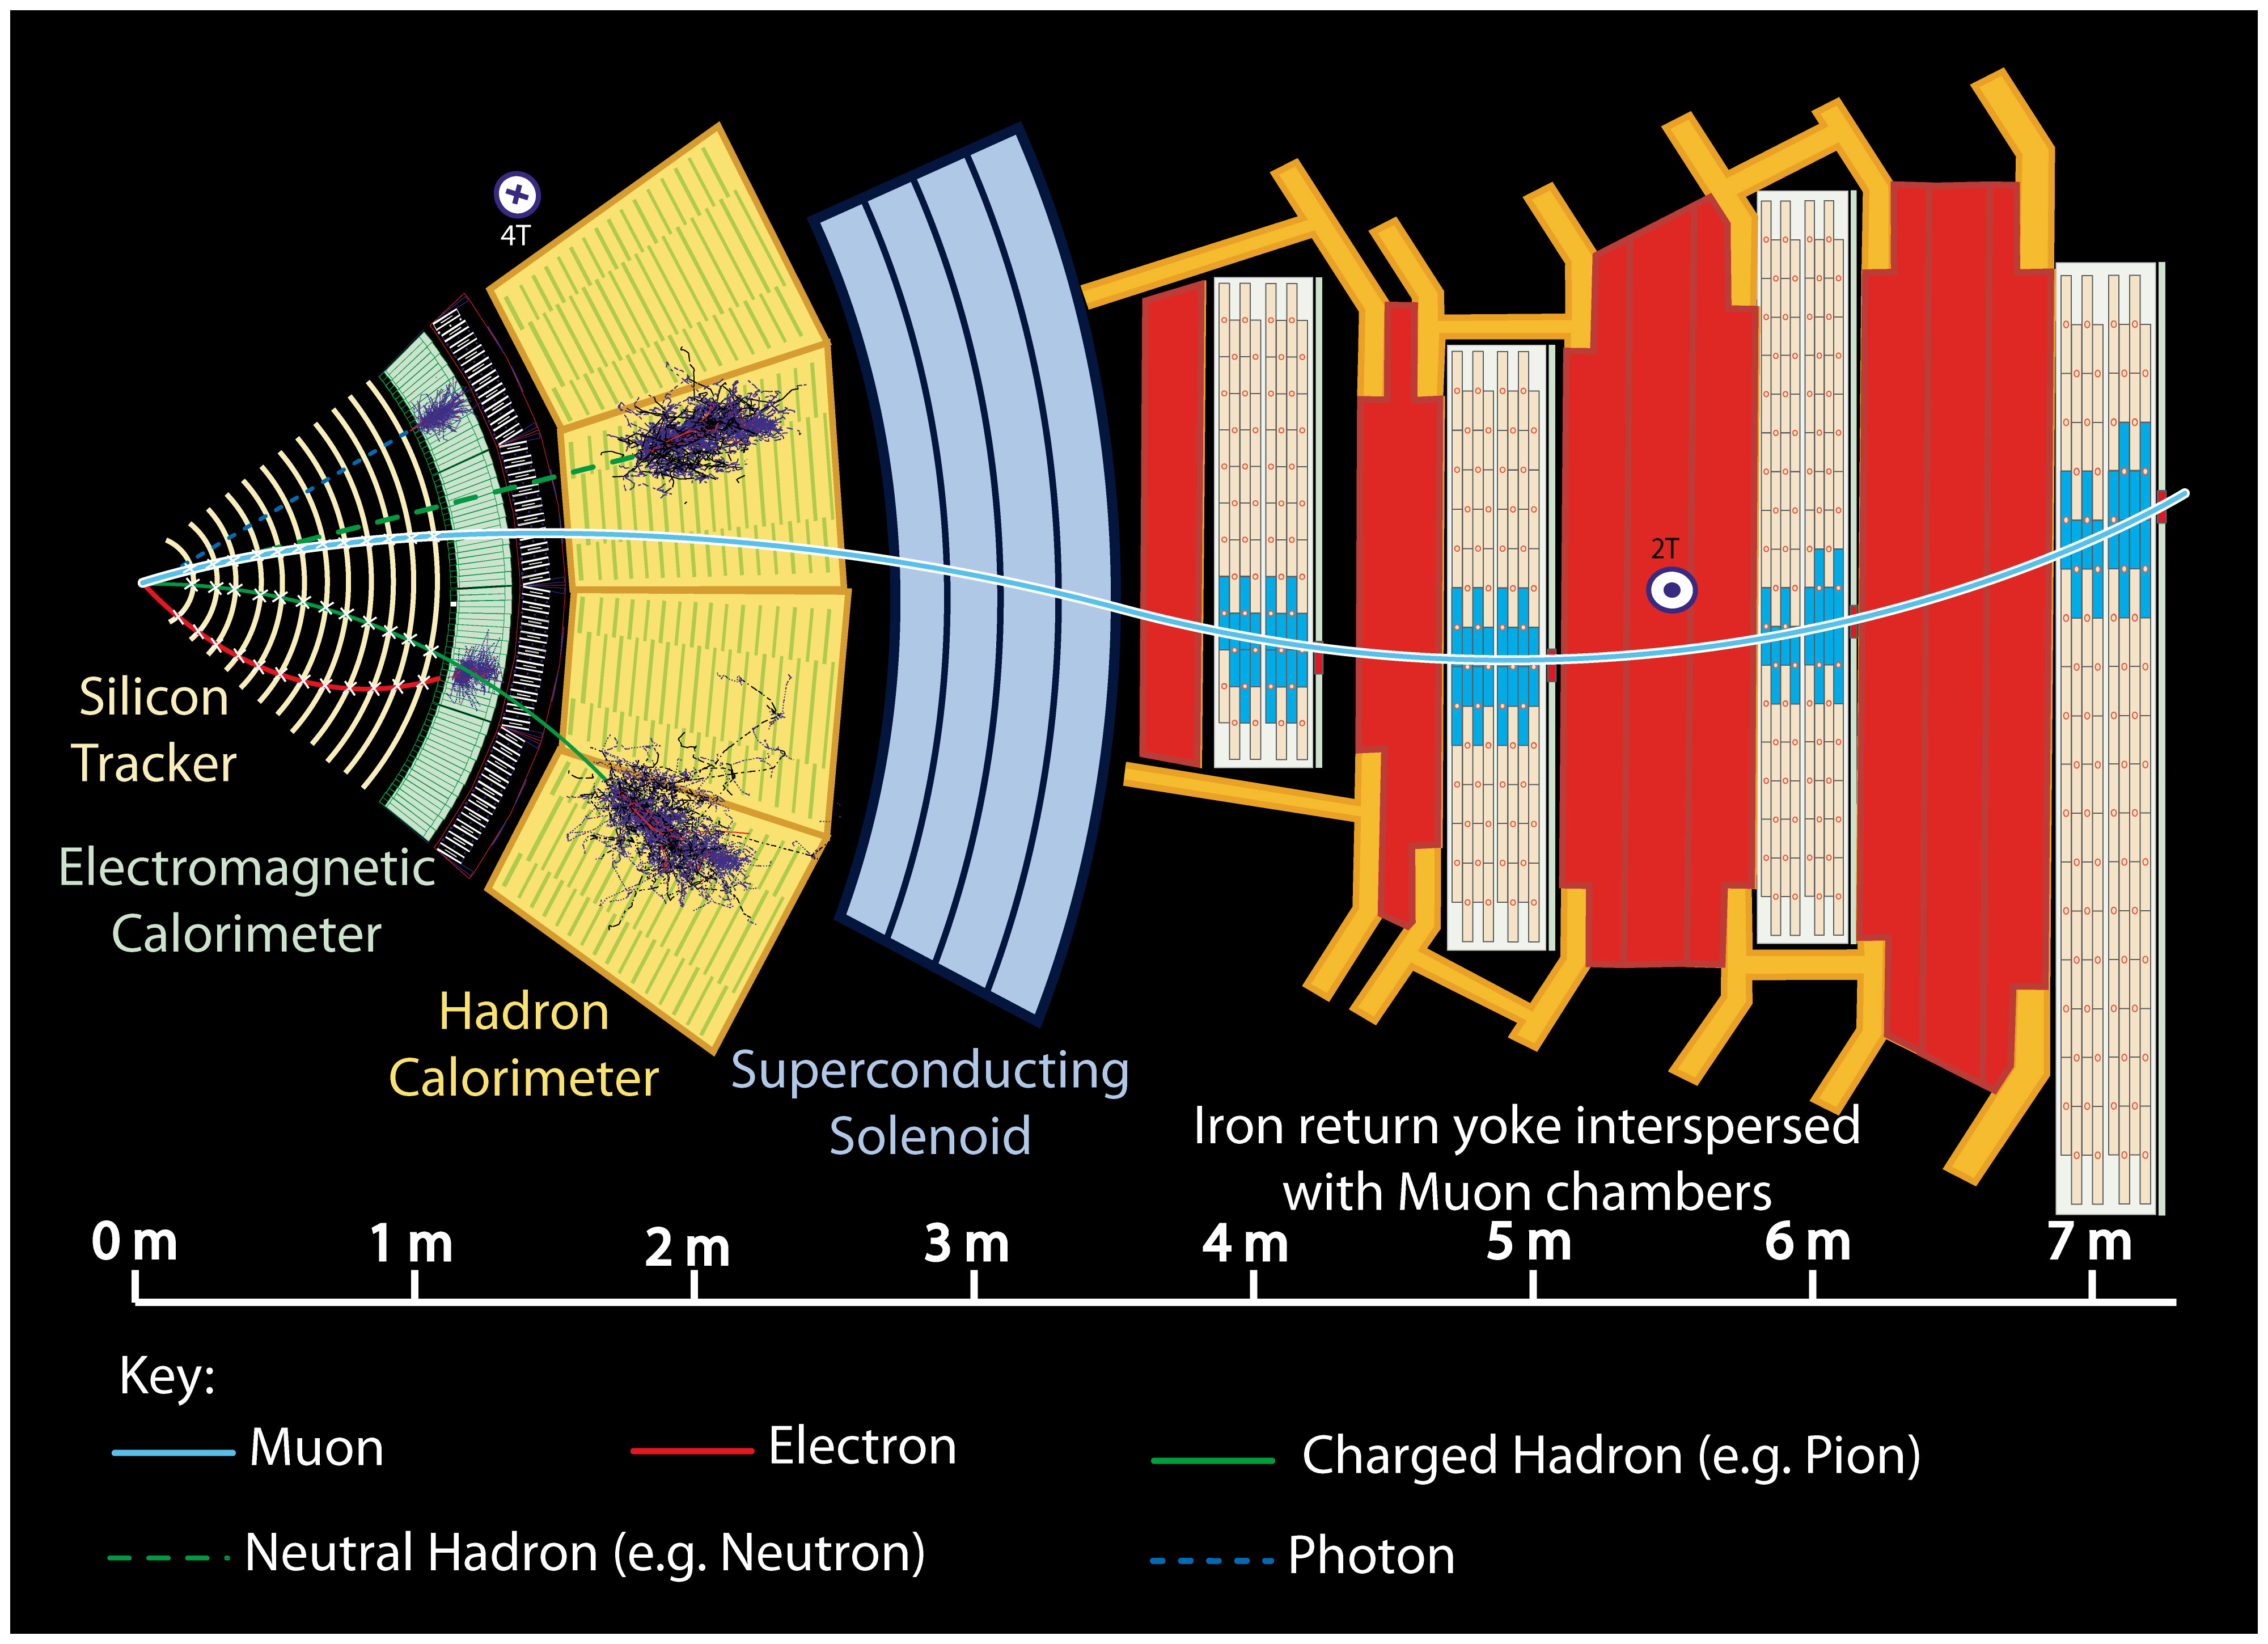
\includegraphics[width=0.7\textwidth]{../figs/PictureforPoint5_oct04_allp.jpg}
    %\caption{CMS sub-detectors and particle identification. }
    %\label{fig:cmsslice}
  \end{center}
\end{figure}
\vspace{-.4cm}
\begin{block}{}
\begin{itemize}\tiny
\item Tracker system: Pixel system (vertex reconstruction) and Silicon strips (Measurement of \pt~of charged particles)
\item Electromagnetic calorimeter (ECAL): 80000 crystals for the measurement of electrons and photons energy
\item Hadron calorimeter (HCAL): Absorber and scintillator to measure the energy of hadrons
\item Muon chambers: RPC, DT and CSC to measure muons \pt
\end{itemize}
\end{block}

\end{frame}


\begin{frame}{}
\vspace{-.2cm}

\begin{textblock}{95}(0,6)
    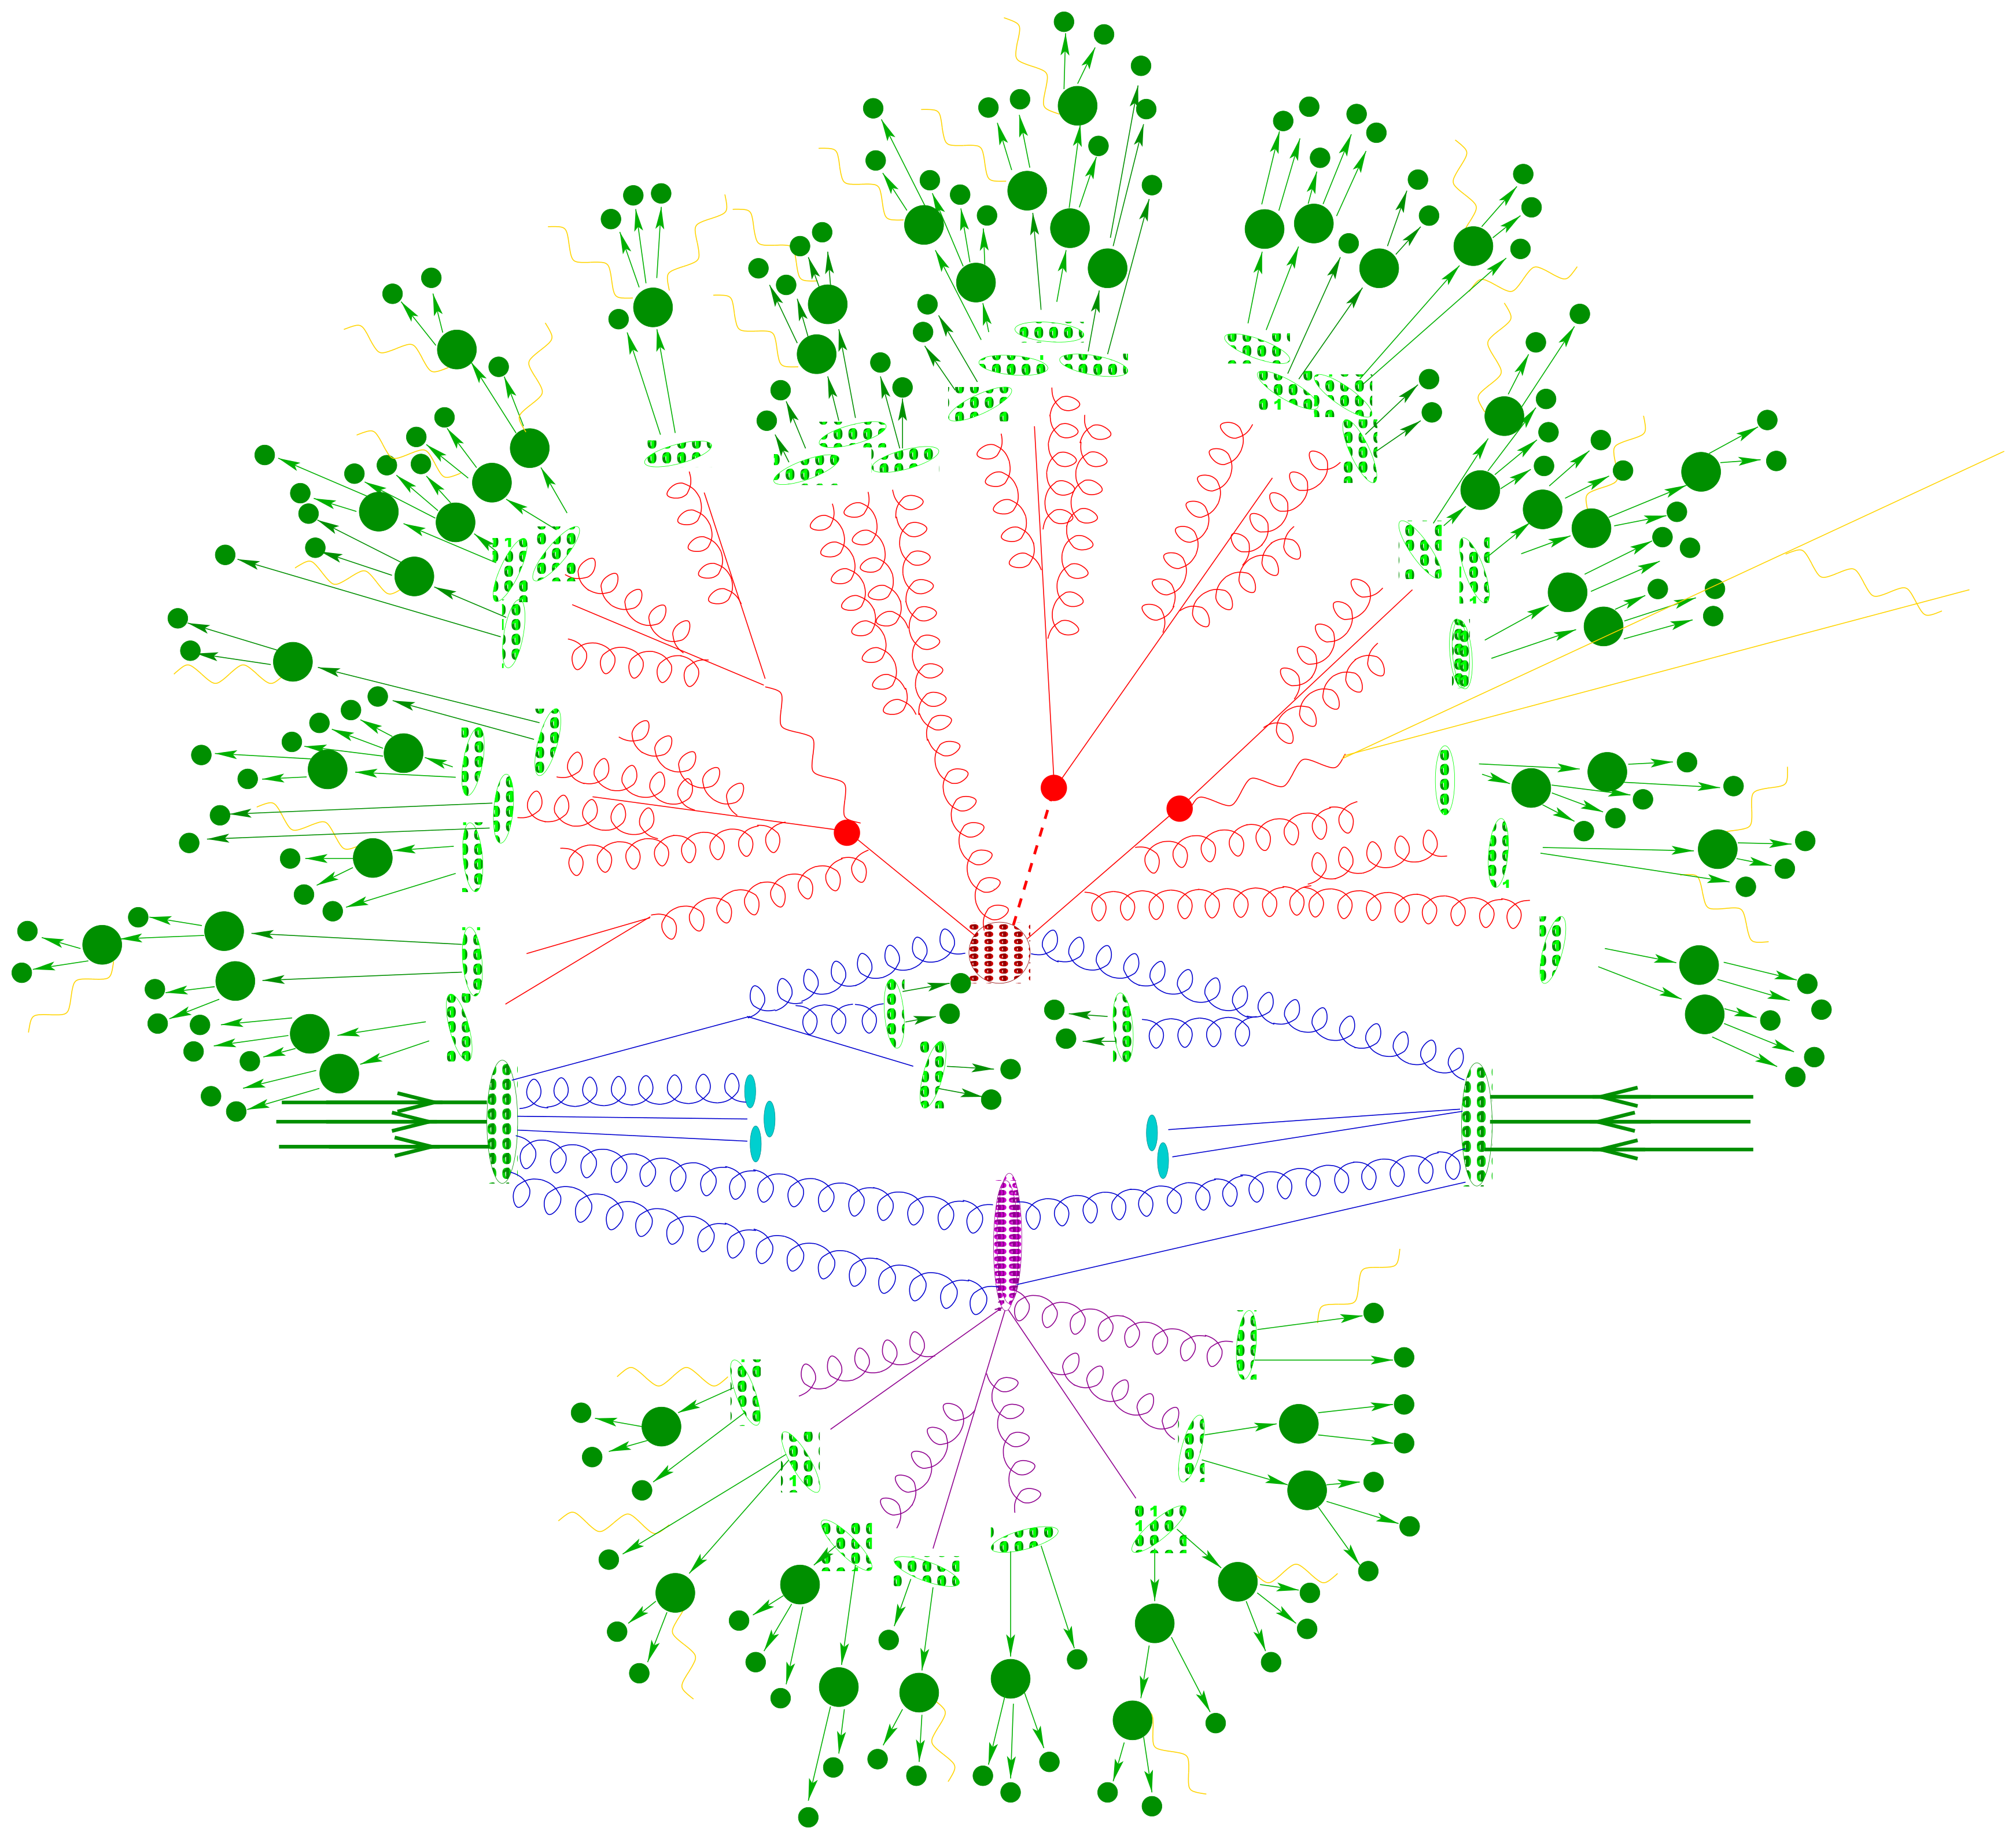
\includegraphics[width=1.0\textwidth]{parton_shower.jpg}
\end{textblock}
\begin{textblock}{40}(90,15)
\includegraphics[width=1.0\textwidth]{Jet_composition_data_7TeV.png}
\end{textblock}
\begin{textblock}{42}(85,55)
\includegraphics[width=1.0\textwidth]{JECUnc.png}
\end{textblock}
%\begin{textblock}{50}(75,70)
%\includegraphics[width=1.0\textwidth]{BTag.png}
%\end{textblock}

\end{frame}


\begin{frame}{B-tagging}
\vspace{-.2cm}

\begin{columns}
\begin{column}{.40\textwidth}
\begin{block}{}\tiny
  \begin{itemize}
  \item Multivariate algorithm to tag b-jets: Combined Secondary Vertex (CSV)
  \item Several jet properties used: \\Number of secondary vertices, flight distance, ...
  \item 3 working points:
    \begin{itemize}\tiny
    \item Loose (CSVL): High b-tagging efficiency, low purity
    \item Medium (CSVM): Medium b-tagging efficiency and purity
    \item Tight (CSVT): High purity, low b-tagging efficiency
    \end{itemize}
  \end{itemize}
\end{block}
\includegraphics[width=1.0\textwidth]{NSV.png}
\end{column}
\begin{column}{.60\textwidth}
\includegraphics[width=1.05\textwidth]{BTag.png}
\end{column}
\end{columns}

\end{frame}

\begin{frame}{}

\includegraphics[width=1.0\textwidth]{/home/jruizalv/Fireworks/cmsShow-5.3/Evt_372.jpg}

\end{frame}

\begin{frame}{Monte-Carlo simulation}
\vspace{-.4cm}
\begin{columns}
\begin{column}{.50\textwidth}
  \begin{block}{MadGraph - MadSpin}\tiny
    Simulation of hard interaction in collisions \\
    \textbf{Figure}: \Z+jets production, \Z~$\to$ neutrinos \MVAt~8 TeV
  \end{block}
\vspace{-.5cm}
\begin{figure}[!Hhtbp]
  \begin{center}
    %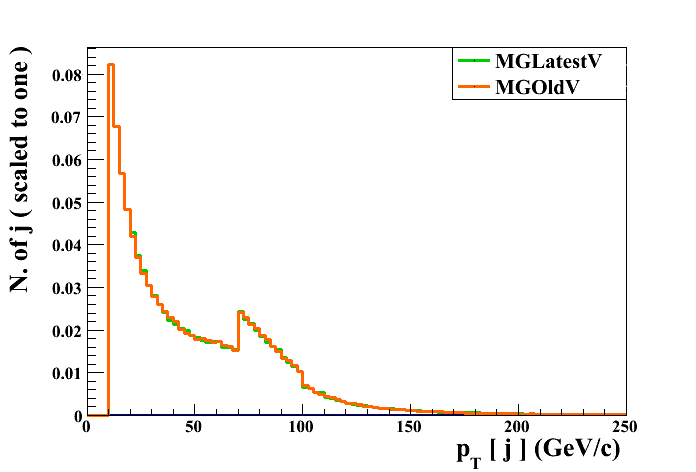
\includegraphics[width=0.9\textwidth]{ZjetsRelVal1.png}\\
    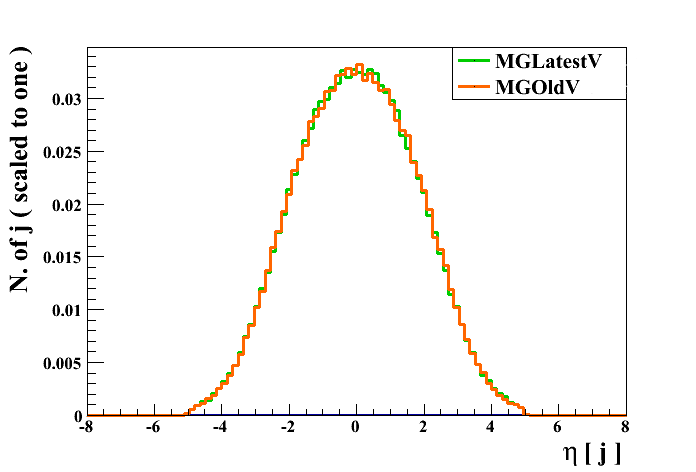
\includegraphics[width=1.0\textwidth]{ZjetsRelVal2.png}
  \end{center}
\end{figure}
\end{column}

\begin{column}{.50\textwidth}
  \begin{block}{RIVET toolkit}\tiny
    \textbf{Pythia}: Simulation of hadronization and showering \\
    Comparison of different generators with real data %\\
    %\textbf{Figure}: \W~boson $p_{T}$ measured by ATLAS experiment in muon final states compared to different MC simulations. py6 stands for Pythia 6, py8 for Pythia 8, MGpy6 MadGraph interfaced with Pythia 6 and PWG for Powheg. MadGraph with Pythia 6 gives the best description of experimental data.
  \end{block}
  \begin{figure}[!Hhtbp]
  \begin{center}
    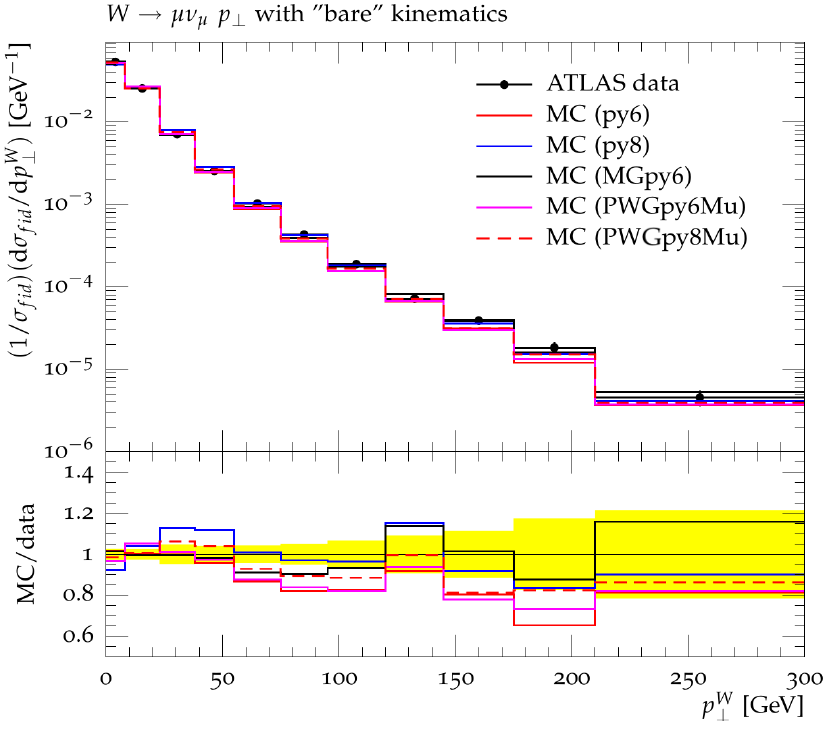
\includegraphics[width=1.0\textwidth]{Wpt_rivet.png}
  \end{center}
\end{figure}
\end{column}
\end{columns}

\end{frame}



\begin{frame}{Interface between partonic and hadronic simulation}
\vspace{-.2cm}
\begin{columns}
\begin{column}{.50\textwidth}
  \begin{block}{}\tiny
    Possible overlap between parton shower and matrix element when adding extra jets. MLM merging:
    \begin{itemize}
    \item $N^{ME}(j)$ \MVAt~parton level
    \item $N^{PS}(j)$ after parton shower
    \item Compare $N^{ME}(j)$ and $N^{PS}(j)$
    \end{itemize}
  \end{block}
\end{column}
\begin{column}{.50\textwidth}
  \begin{block}{}\tiny
    To study the correctness of the choice:
    \begin{itemize}
    \item DJR diagrams
    \item Transition between $n$ and $n-1$ jet multiplicities as a function of the merging scale
    \end{itemize}
  \end{block}
\end{column}
\end{columns}

\vspace{-.2cm}
\begin{columns}
\begin{column}{.30\textwidth}
\begin{figure}[!Hhtbp]
  \begin{center}
    \includegraphics[width=1.3\textwidth]{ExplainDJR.png}
  \end{center}
\end{figure}
\end{column}
\begin{column}{.70\textwidth}
\begin{figure}[!Hhtbp]
  \begin{center}
    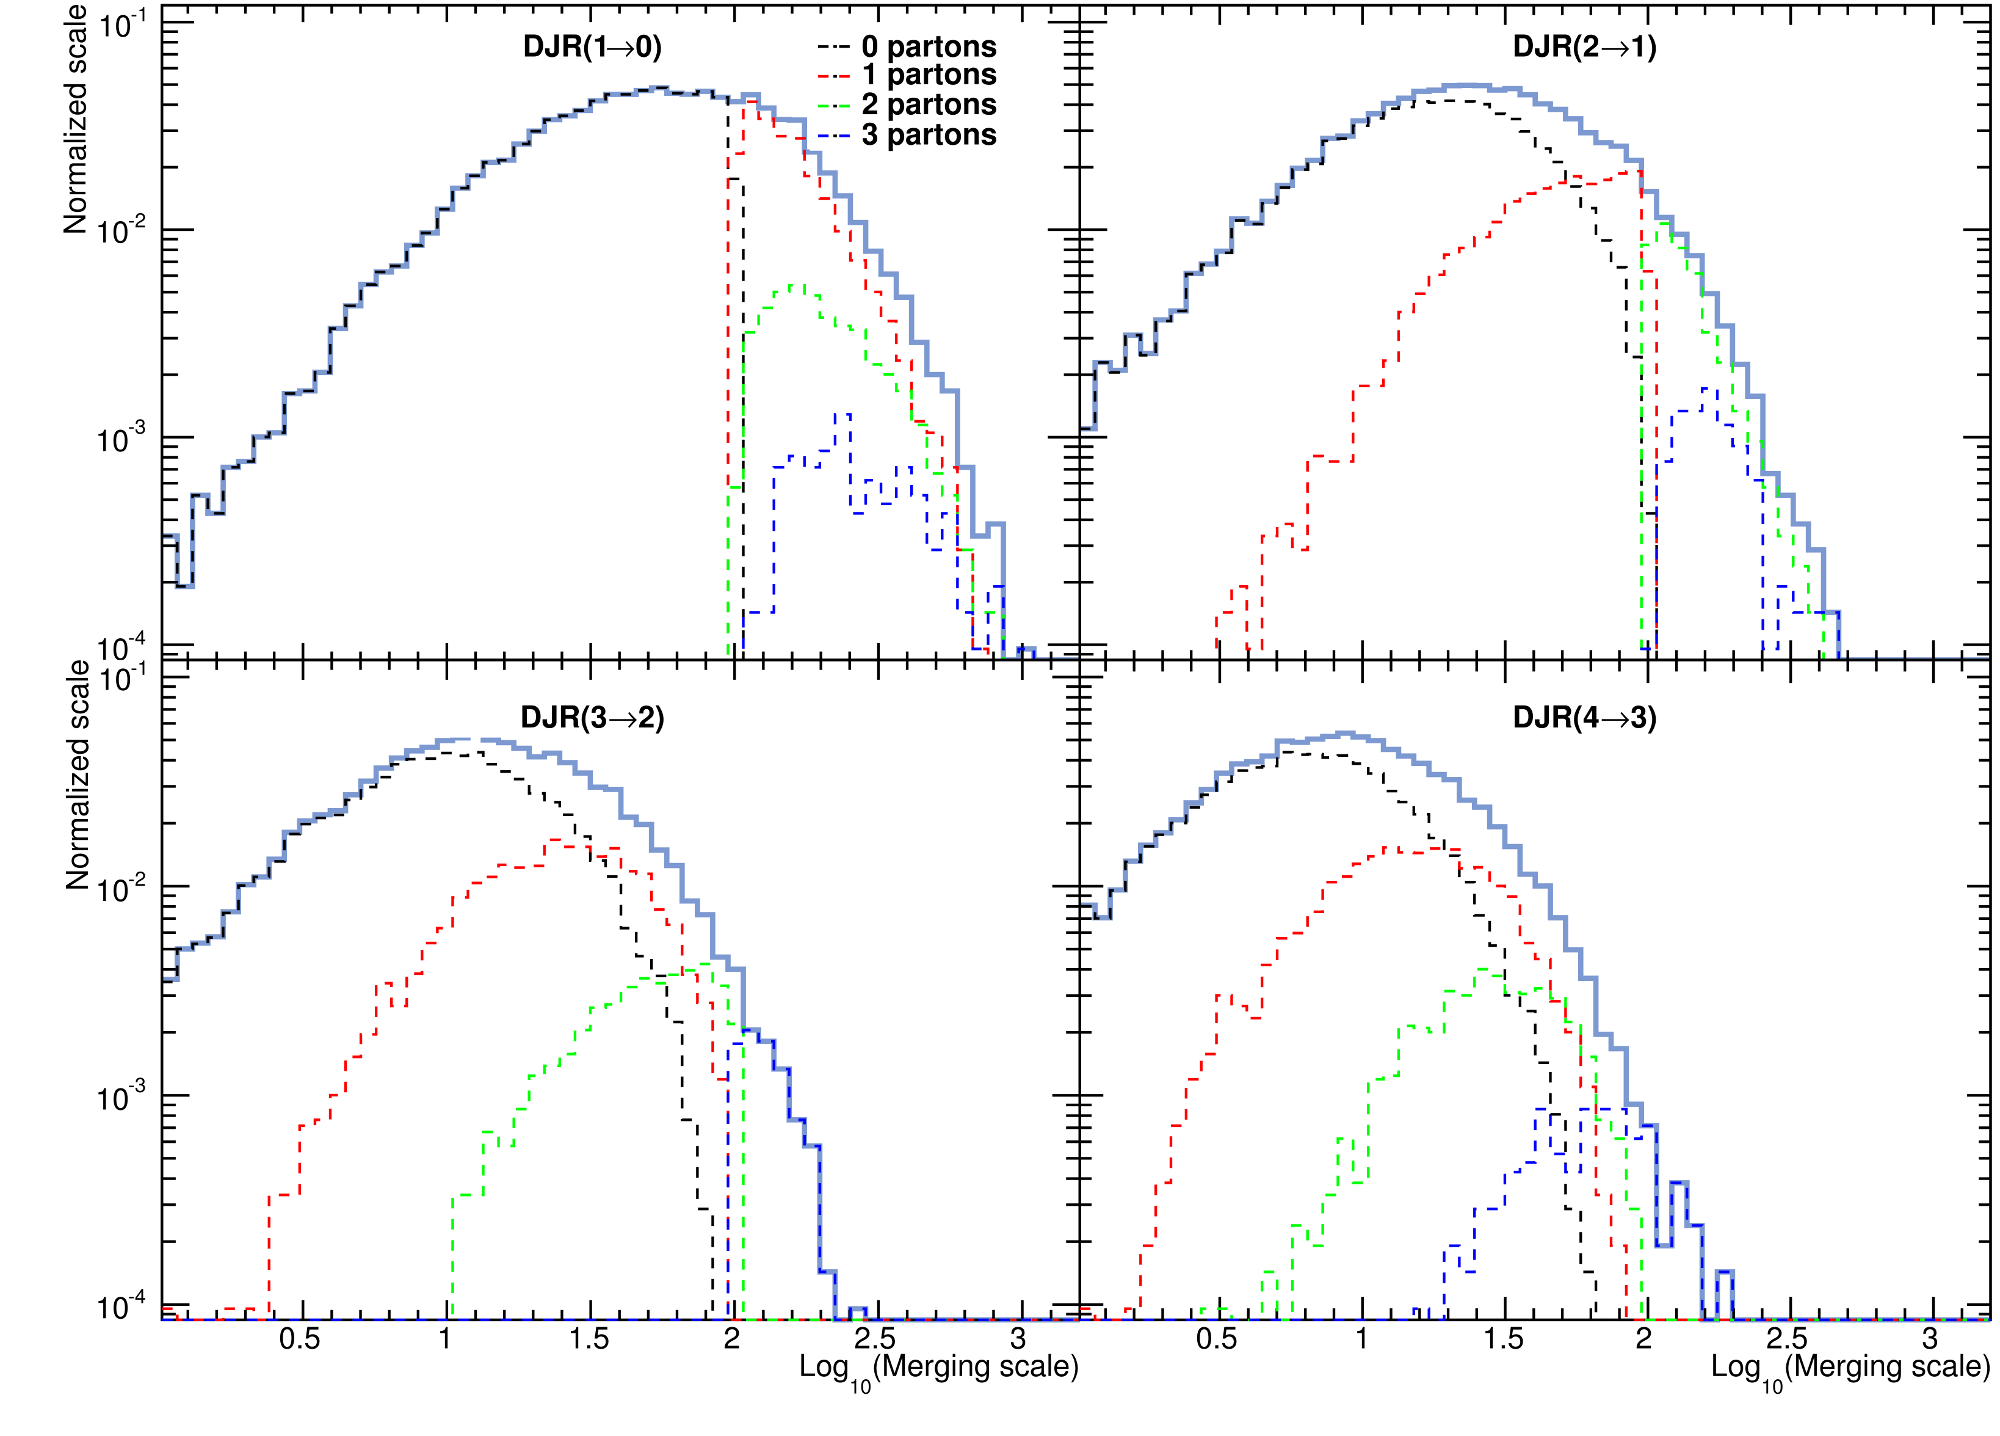
\includegraphics[width=1.0\textwidth]{../figs/DJR_q100_xq20_TTJets13TeV.png}
  \end{center}
\end{figure}
\end{column}
\end{columns}


%\begin{figure}[!Hhtbp]
%  \begin{center}
%    \includegraphics[width=0.3\textwidth]{ExplainDJR.png}
%    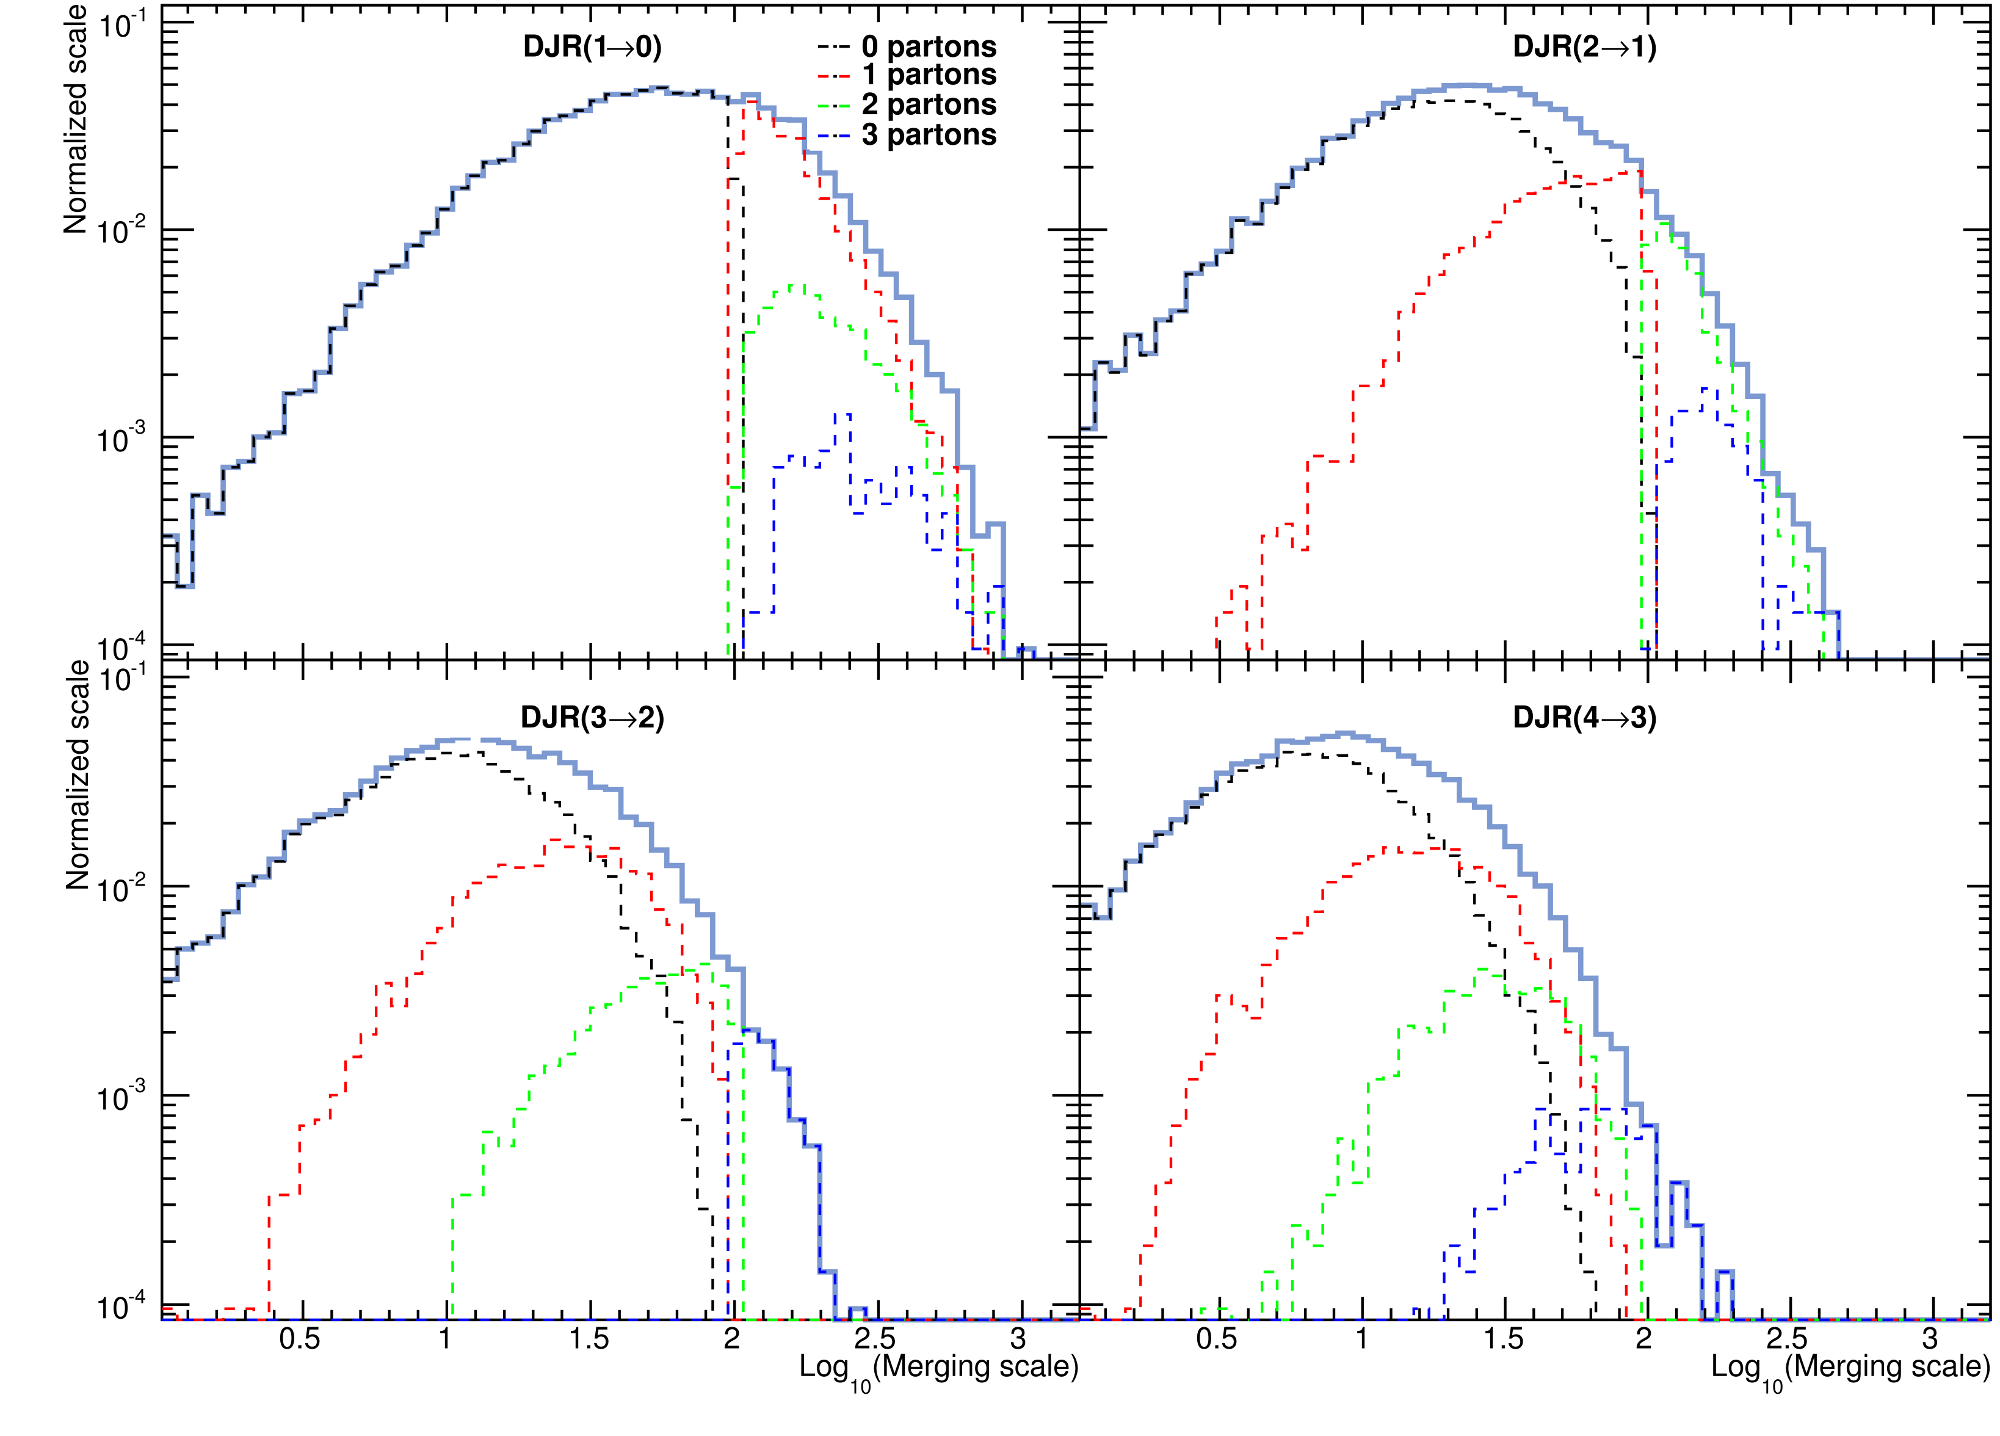
\includegraphics[width=0.7\textwidth]{../figs/DJR_q100_xq20_TTJets13TeV.png}
    %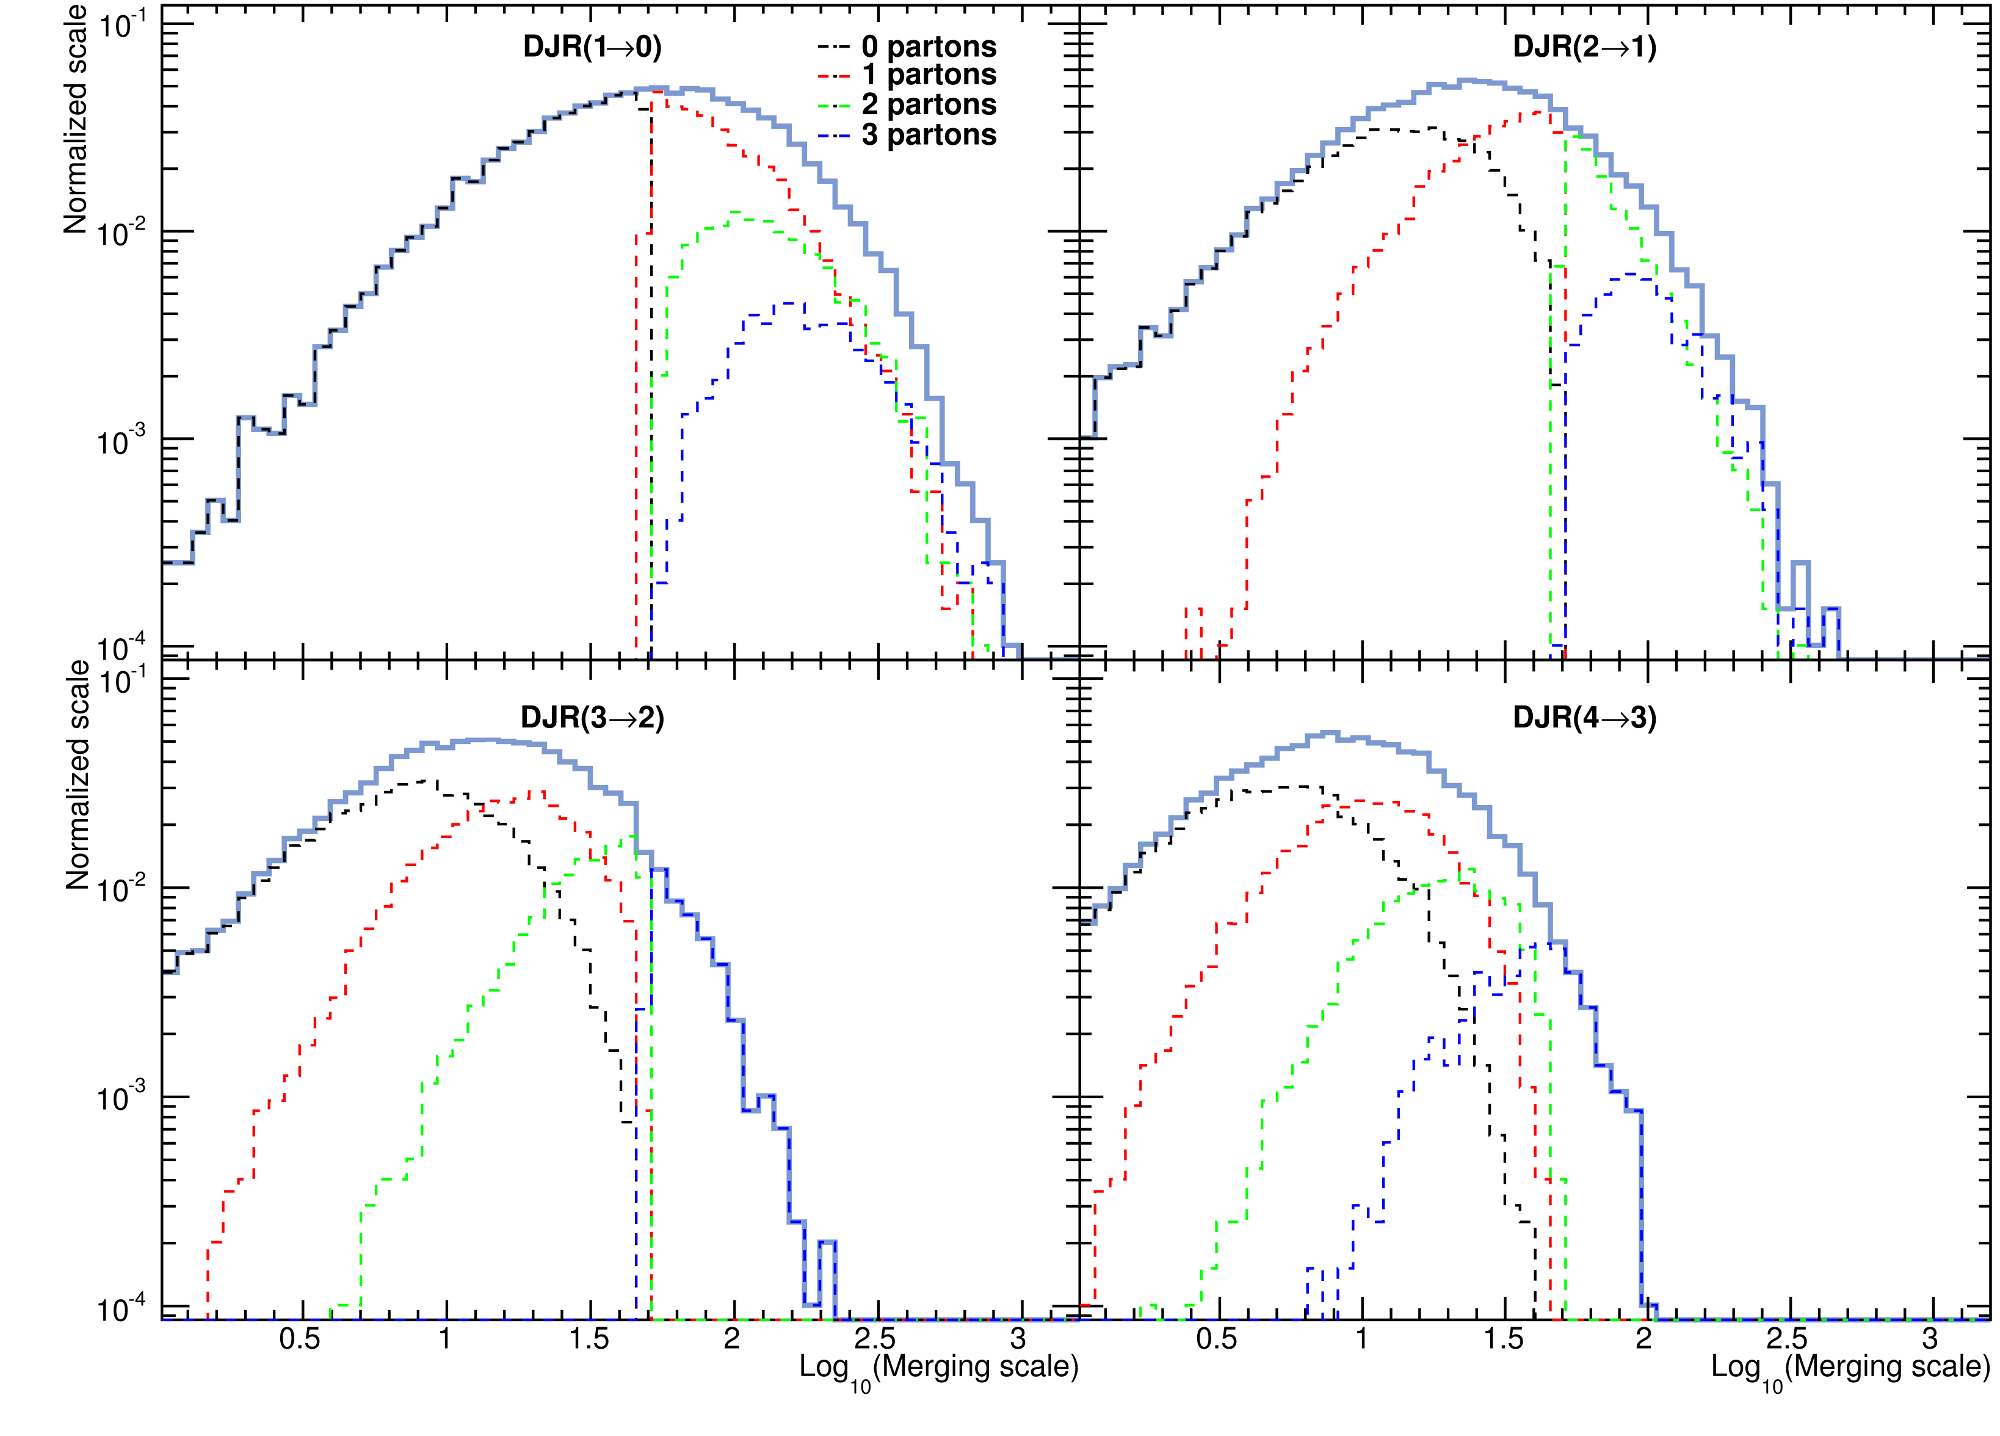
\includegraphics[width=0.5\textwidth]{../figs/DJR_q50_xq20_TTJets13TeV.png}
    %\caption{DJR diagrams for 13 TeV top pair production with $Q_{cut}=100$ GeV and $Q^{X}_{cut}=20$ GeV [optimal case] (top) and $Q_{cut}=60$ GeV and $Q^{X}_{cut}=20$ [non-optimal] (bottom). Bottom figure shows a discontinuity in the transition from 3 to 2 partons at the point where blue-dashed and green-dashed curves meet.}
    %\label{fig:TTJetsMerging}
%  \end{center}
%\end{figure}
%
%\vspace{-.2cm}
%  \begin{block}{}\tiny
%    \textbf{Figure}: DJR diagrams for 13 TeV top pair production with $Q_{cut}=100$ GeV and $Q^{X}_{cut}=20$ GeV [optimal case] (left) and $Q_{cut}=60$ GeV and $Q^{X}_{cut}=20$ [non-optimal] (right). Right figure shows a discontinuity in the transition from 3 to 2 partons at the point where blue-dashed and green-dashed curves meet.
%  \end{block}

\end{frame}


\iffalse
\begin{frame}{CMS: Compact Muon Solenoid}
\vspace{-.2cm}

\begin{columns}
\begin{column}{.30\textwidth}
\begin{block}{}
\begin{itemize}\scriptsize
\item One of two general purpose experiments of LHC
\item Cylinder of 28.7 m long and 15 m height and 14000 tons
\end{itemize}
\tiny{
\begin{equation*}  
\eta = -\text{ln}\left( \text{tan}\left(\frac{\theta}{2}\right)\right)
\end{equation*}
\begin{equation*}
\Delta R=\sqrt{(\Delta\eta)^{2}+(\Delta\phi)^{2}}
\end{equation*}
}%
\end{block}
\end{column}

\begin{column}{.70\textwidth}
\begin{figure}[!Hhtbp]
  \begin{center}
    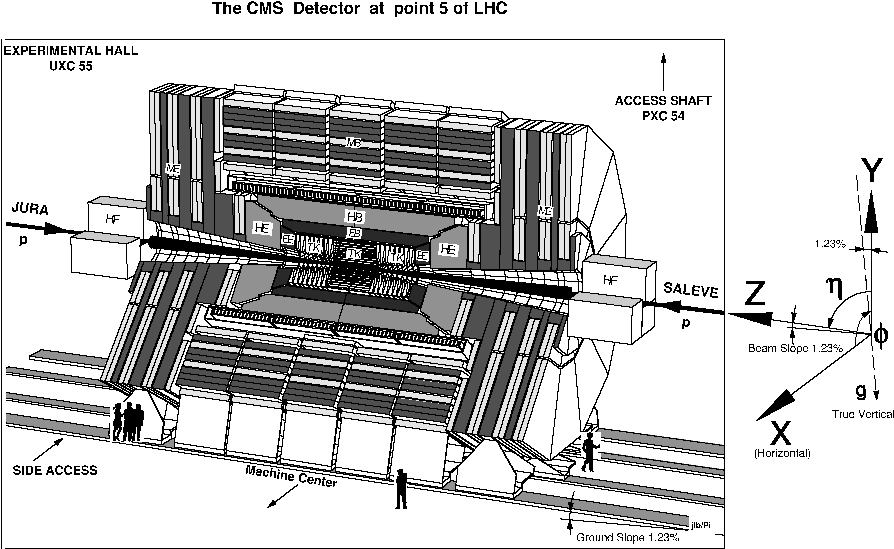
\includegraphics[width=\textwidth]{../figs/CMS_coordinates.jpg}
  \end{center}
\end{figure}
\end{column}
\end{columns}

\vspace{-.2cm}
\begin{block}{}
\begin{itemize}\scriptsize
\item Compact: The calorimeters are inside the magnet
\item Muon: Very precise measurement of muons
\item Solenoid: Solenoidal magnet of 3.8 T magnetic field
\end{itemize}
\end{block}

\end{frame}


\begin{frame}{Sub-detectors}
\vspace{-.2cm}
\begin{figure}[!Hhtbp]
  \begin{center}
    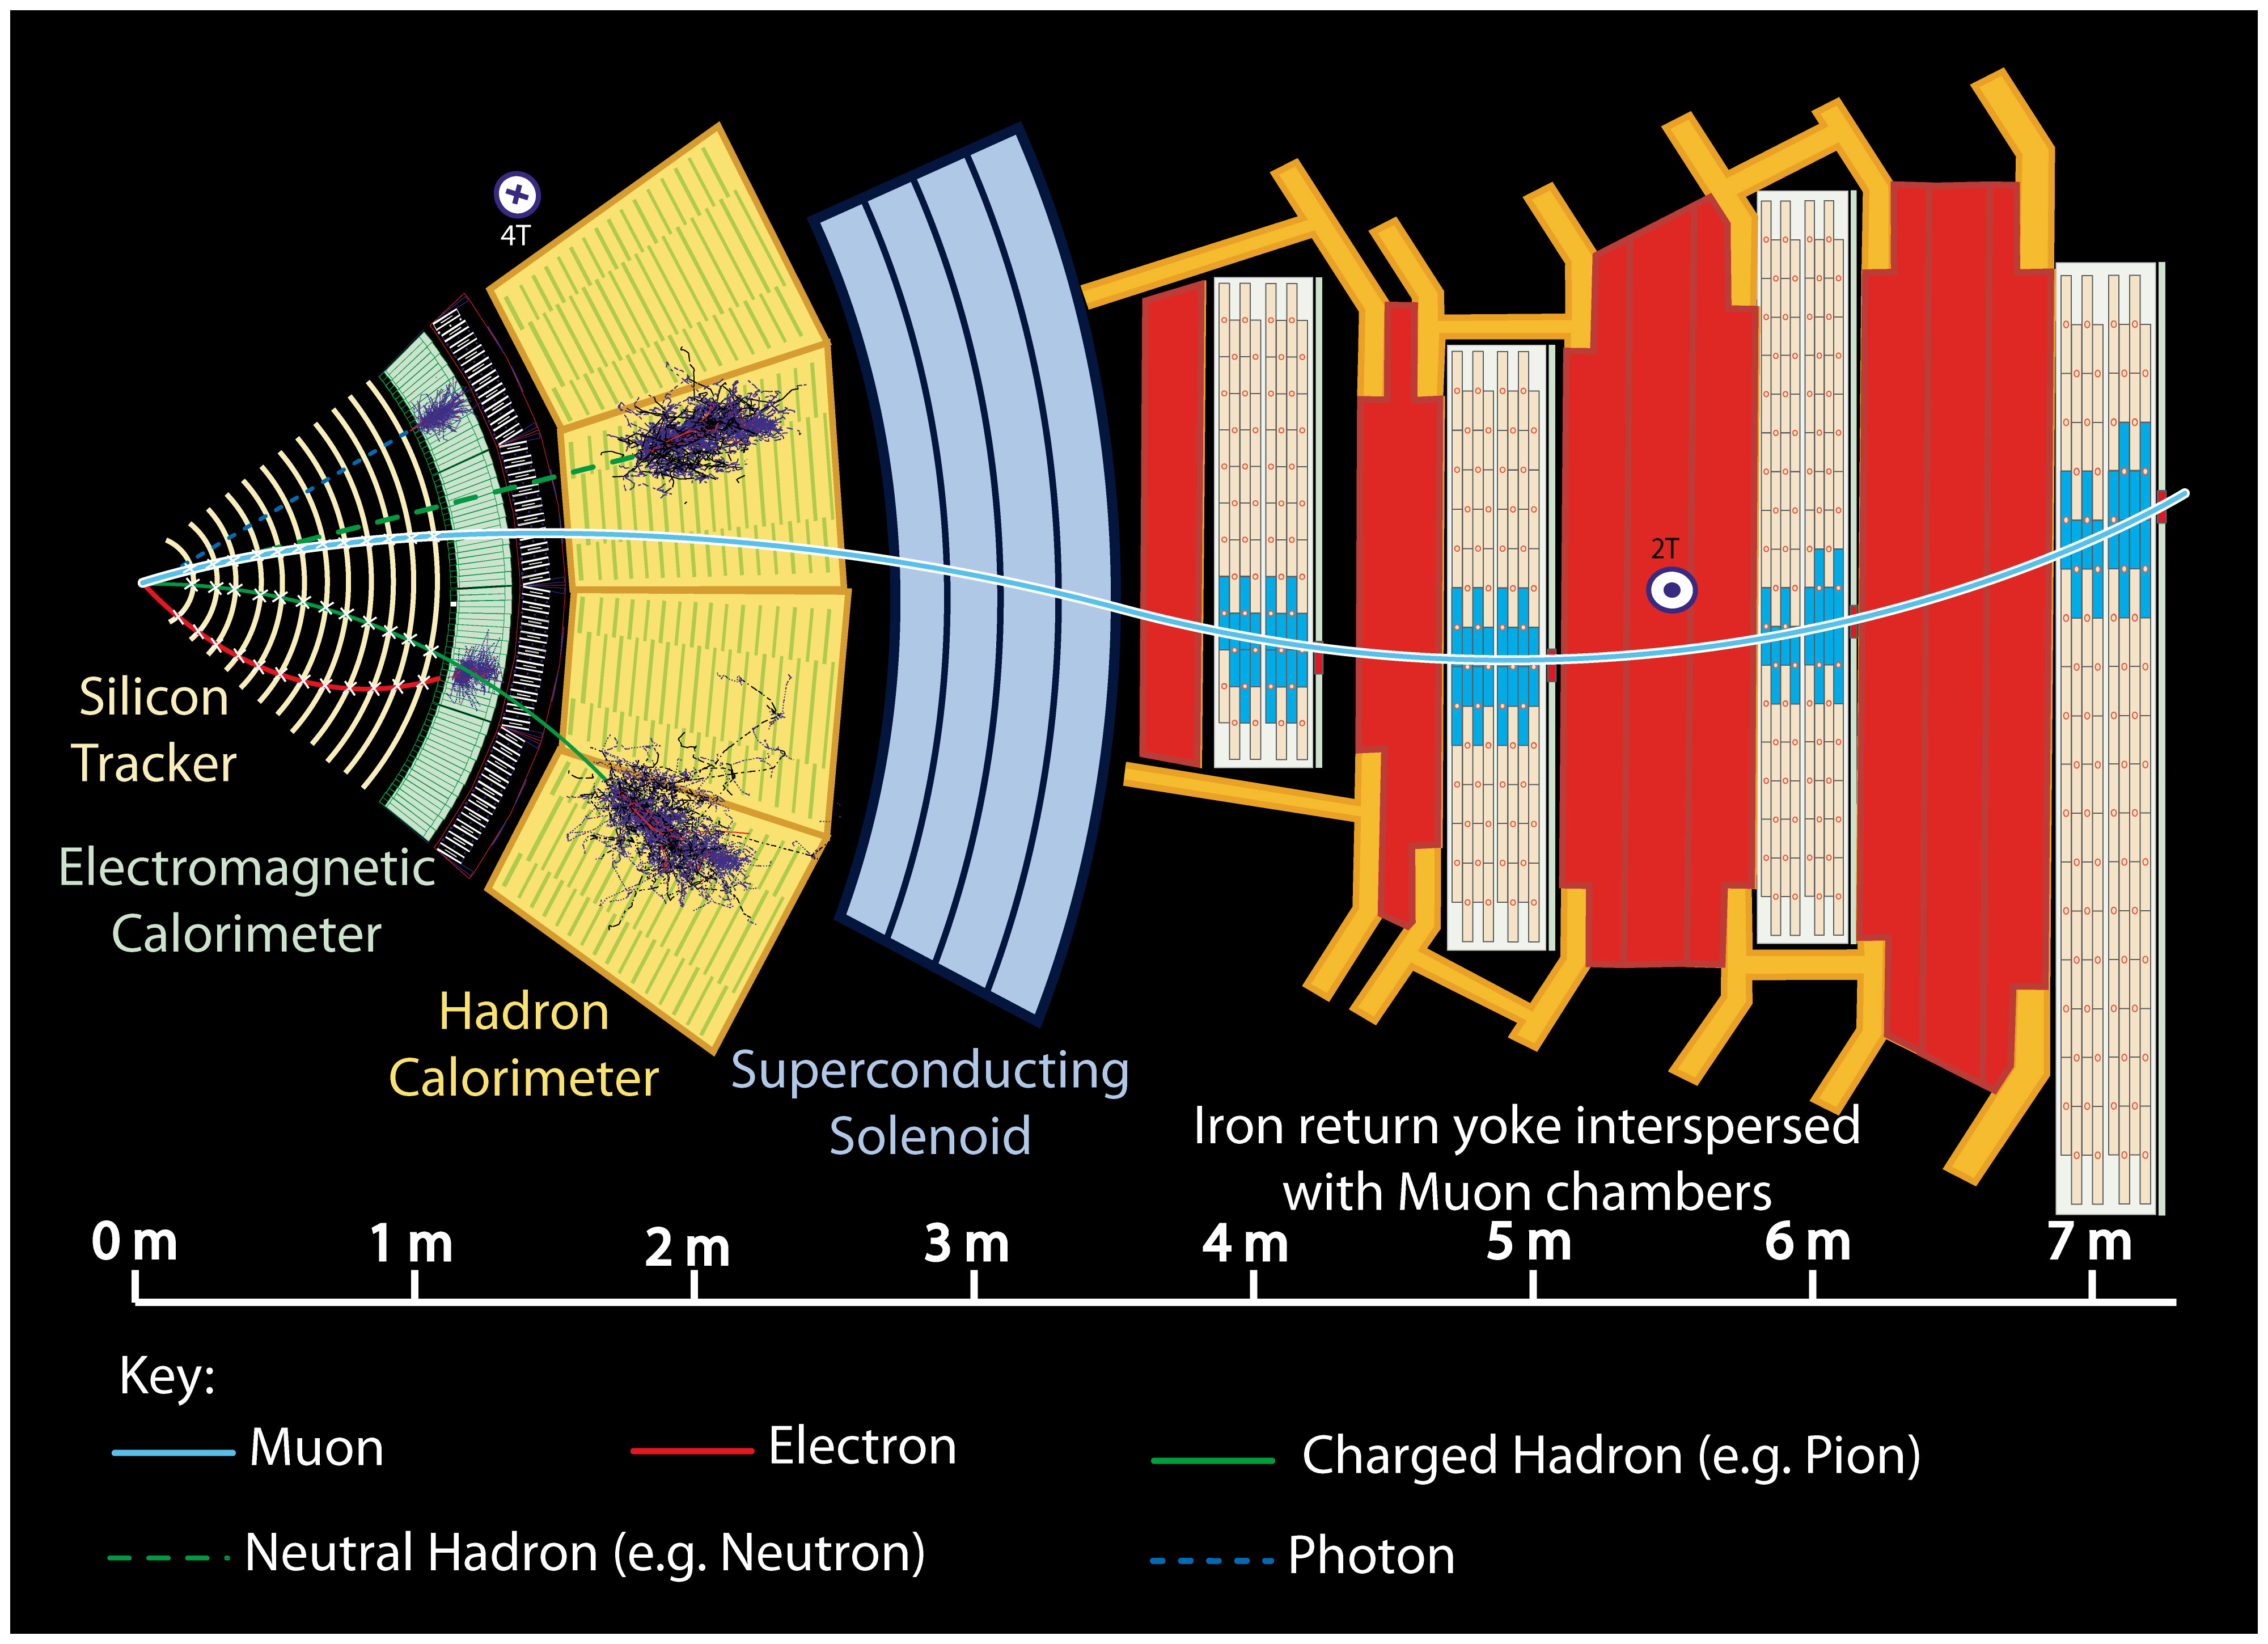
\includegraphics[width=0.7\textwidth]{../figs/PictureforPoint5_oct04_allp.jpg}
    %\caption{CMS sub-detectors and particle identification. }
    %\label{fig:cmsslice}
  \end{center}
\end{figure}
\vspace{-.4cm}
\begin{block}{}
\begin{itemize}\tiny
\item Tracker system: Pixel system (vertex reconstruction) and Silicon strips (Measurement of \pt~of charged particles)
\item Electromagnetic calorimeter (ECAL): 80000 crystals for the measurement of electrons and photons energy
\item Hadron calorimeter (HCAL): Absorber and scintillator to measure the energy of hadrons
\item Muon chambers: RPC, DT and CSC to measure muons \pt
\end{itemize}
\end{block}

\end{frame}


\begin{frame}{Object reconstruction - Jets}
\vspace{-.9cm}

\begin{columns}
\begin{column}{.55\textwidth}
\begin{block}{}
\begin{itemize}\tiny
\item Tracker information is used to reconstruct charged particles $\to$ Charged hadrons, electrons, muons
\item ECAL + HCAL information used to reconstruct the energy of hadrons (neutral and charged)
\item Tracker system + ECAL + HCAL information are combined to reconstruct jets $\to$ objects used to recover the information from a quark or gluon produced in the hard scattering
\item Several algorithms are used to collect all reconstructed particles in a jet: CMS $\to$ anti-kt algorithm with a radius $R=0.5$ (AK5)
\item Jet energy measurement can suffer of missing tracks, pile-up or other detector effects $\to$ Strategies needed to correct jet energy 
\item Jet energy information is analyzed by an MVA algorithm to determine if it was produced by a b quark $\to$ Constrained Secondary Vertex (CSV) discriminator for b-jets in three working points:\\
\tiny{
\textbf{CSVL (Loose)}: Discriminator > 0.244, $\epsilon^{CSVL}_{b}=85$\%, $\epsilon^{CSVL}_{c}=45$\%, $\epsilon^{CSVL}_{l}=10$\%\\
\textbf{CSVM (Medium)}: Discriminator > 0.679, $\epsilon^{CSVM}_{b}=$70\%, $\epsilon^{CSVM}_{c}=$20\%, $\epsilon^{CSVM}_{l}=$1\%\\
\textbf{CSVT (Tight)}: Discriminator > 0.898, $\epsilon^{CSVT}_{b}=50$\%, $\epsilon^{CSVT}_{c}=7$\%, $\epsilon^{CSVT}_{l}=0.2$\%\\
}%
\end{itemize}
\end{block}
\end{column}

\begin{column}{.45\textwidth}
\begin{figure}[!Hhtbp]
\begin{center}
\includegraphics[width=0.6\textwidth,height=0.33\textheight]{../figs/Jet_composition_data_7TeV.png}
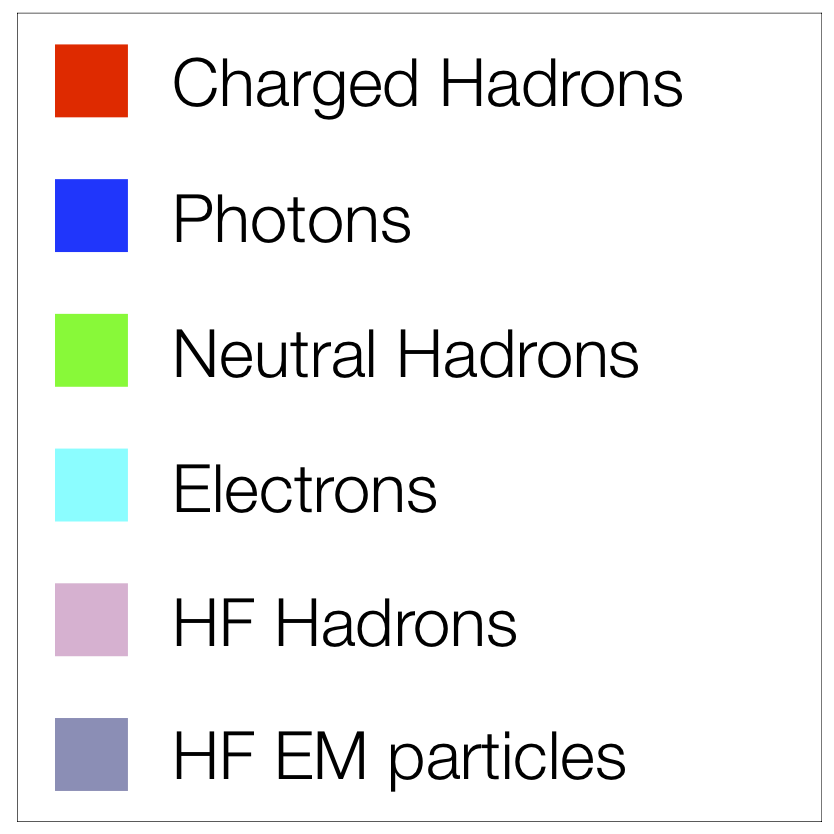
\includegraphics[width=0.3\textwidth]{../figs/Legend_jet_composition.png}\\
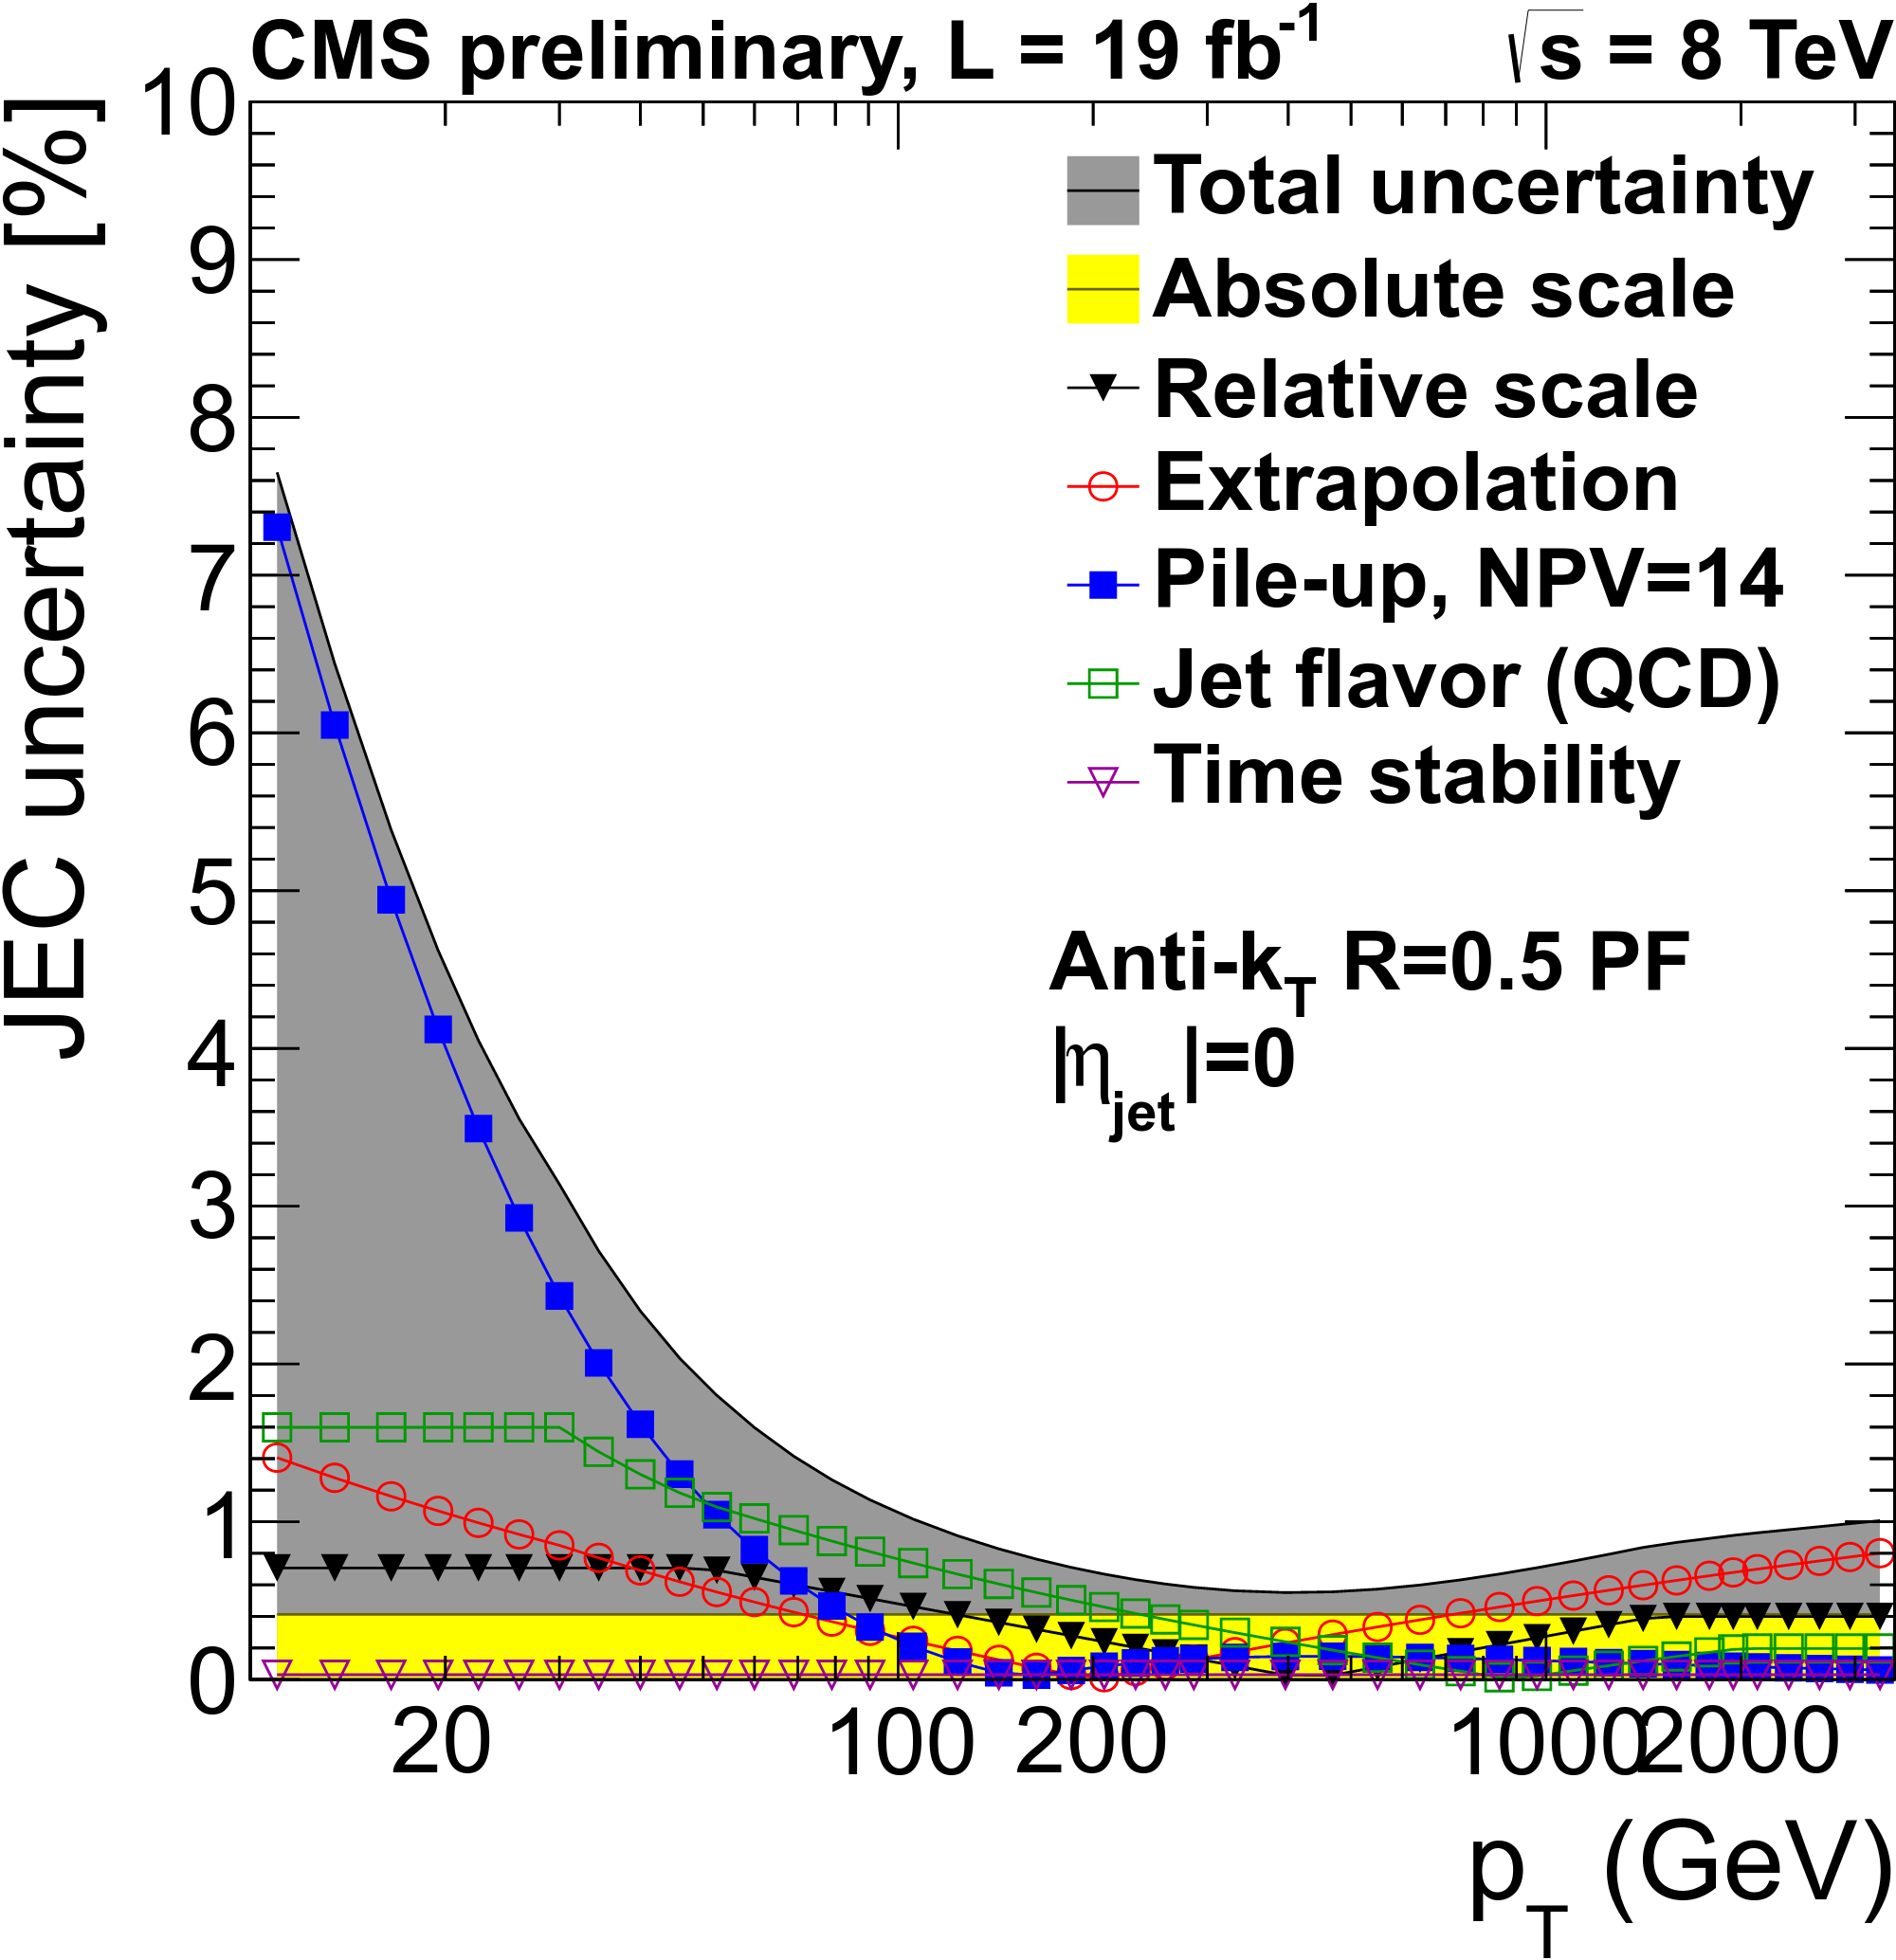
\includegraphics[width=0.55\textwidth,height=0.33\textheight]{../figs/JEC_pt.png}\\
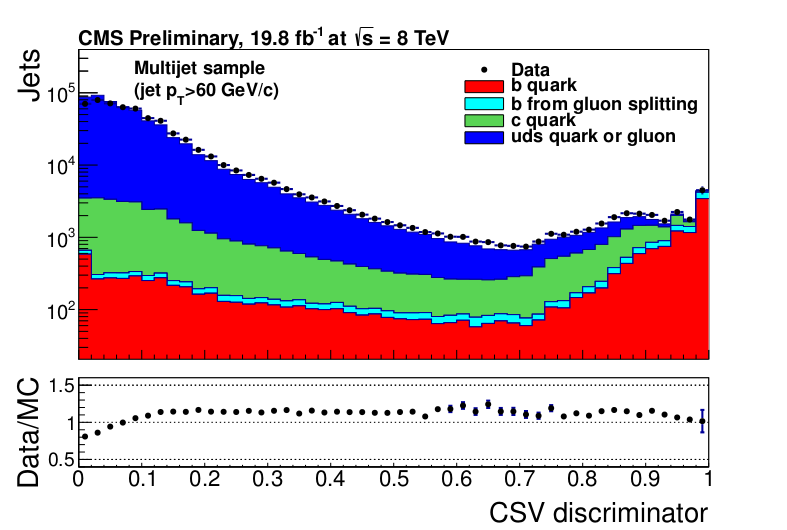
\includegraphics[width=0.6\textwidth,height=0.33\textheight]{../figs/pdf-sub.png}
\end{center}
\end{figure}
\end{column}
\end{columns}

\end{frame}

\fi